\documentclass{article}
\usepackage{tikz}
\usetikzlibrary{shapes.geometric, positioning}
\begin{document}
\begin{enumerate}
\item  The circuit shown in the figure functions as which one of the following digital circuit block?\\
\centering
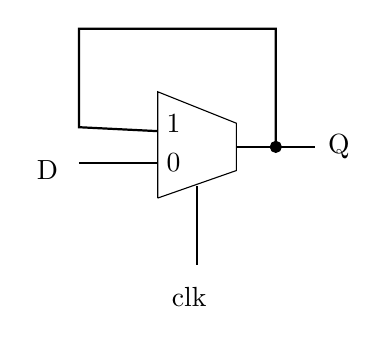
\begin{tikzpicture}
\draw (0,-0.15)--(0,1.2)--(1,0.8)--(1,0.2)--(0,-0.15);
\filldraw (1.5,0.5) circle (2pt);
\draw[thick] (0,0.7) -- (-1,0.75)-- (-1,2) --(1.5,2) --(1.5,0.50);
    \draw[thick] (-1,0.3) -- (0,0.3); % D input
    \draw[thick] (1,0.5) -- (2,0.5); % Q output
    \draw[thick] (0.5,0) -- (0.5,-1); % Clock input
    \node at (-1.4,0.2) {D};
    \node at (2.3,0.5) {Q};
    \node at (0.4,-1.4) {clk};
	\node at (1.2,0.4) {} ;
    \node at (0.2, 0.8) {1};
    \node at (0.2, 0.3) {0};
\end{tikzpicture}
	\hfill{GATE BM 2024}
\begin{enumerate}
\item Negative level triggered D-latch
\item Positive level triggered D-latch
\item Negative edge triggered D-Flipflop
\item Positive edge triggered D-Flipflop
\end{enumerate}
\end{enumerate}
\end{document}
